% presentation.tex
% Matthew Monaco
% Andy Sayler
% Landon Spear

\documentclass[xcolor=dvipsnames]{beamer}
\usetheme{AnnArbor}
\usecolortheme{beaver}
\setbeamercovered{transparent=25}
\setbeamertemplate{blocks}[rounded][shadow=false] 
\setbeamertemplate{navigation symbols}{}

\usepackage{graphicx}
\usepackage{url}
\usepackage{listings}

\bibliographystyle{plain}

\lstloadlanguages{C}
\lstset{
  language=C,
  basicstyle=\footnotesize,
  numbers=none,
  numberstyle=\footnotesize,
  stepnumber=1,
  numbersep=5pt,
  showspaces=false,
  showstringspaces=false,
  showtabs=false,
  tabsize=4,
  captionpos=b,
  breaklines=true,
  breakatwhitespace=false,
  title=\lstname,
  frame=single,
  frameround=tttt
}

\newenvironment{packed_enum}{
\begin{enumerate}
  \setlength{\itemsep}{1pt}
  \setlength{\parskip}{0pt}
  \setlength{\parsep}{0pt}
}{\end{enumerate}}

\newenvironment{packed_item}{
\begin{itemize}
  \setlength{\itemsep}{1pt}
  \setlength{\parskip}{0pt}
  \setlength{\parsep}{0pt}
}{\end{itemize}}

\title[NCD]{Networked Character Devices}
%\subtitle[]{}
\author[Monaco, Sayler, Spear]{Matthew Monaco \&
                               Andrew Sayler \&
                               Landon Spear}
\institute[CU-Boulder]{
  University of Colorado at Boulder \\
  \texttt{\{first.last\}@colorado.edu}
}
\date[Dec. 10, 2011]{Saturday, December 10\textsuperscript{th}, 2011}

\begin{document}

%---Title Slide---%
\begin{frame}[plain]
  \titlepage
\end{frame}

\begin{frame}{Outline}
  \tableofcontents
\end{frame}

%Landon - Beginning

\section{Overview}
%---Intro Slide---%
\begin{frame}{\bf NCD Overview}
  We did some stuff, we used some references \cite{ldd3}.
\end{frame}

\section{Introduction}

\section{Related Work}

% Matt - Middle

% Combine Architecture and System?
\section{Architecture}

\begin{frame}[c]{Very High Level}
  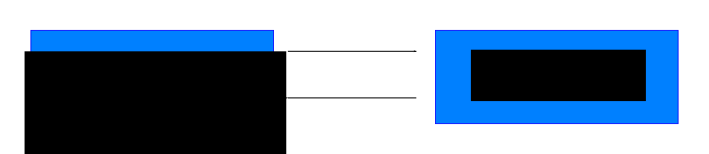
\includegraphics[width=0.8\textwidth]{arch-01.png}

  \begin{itemize}
    \item<1-> Our system uses a basic client server model
    \item<2-> The client initiates all exchanges, the server replies
  \end{itemize}
\end{frame}

\begin{frame}[c]{High Level}
  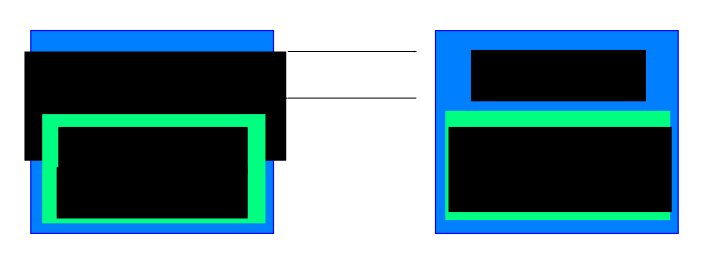
\includegraphics[width=0.8\textwidth]{arch-02.png}

  \begin{itemize}
    \item<1-> The server side resides entirely in a single kernel module
    \item<2-> The client side is a standard userspace server
  \end{itemize}
\end{frame}

\begin{frame}[c]{Client Medium Level}
  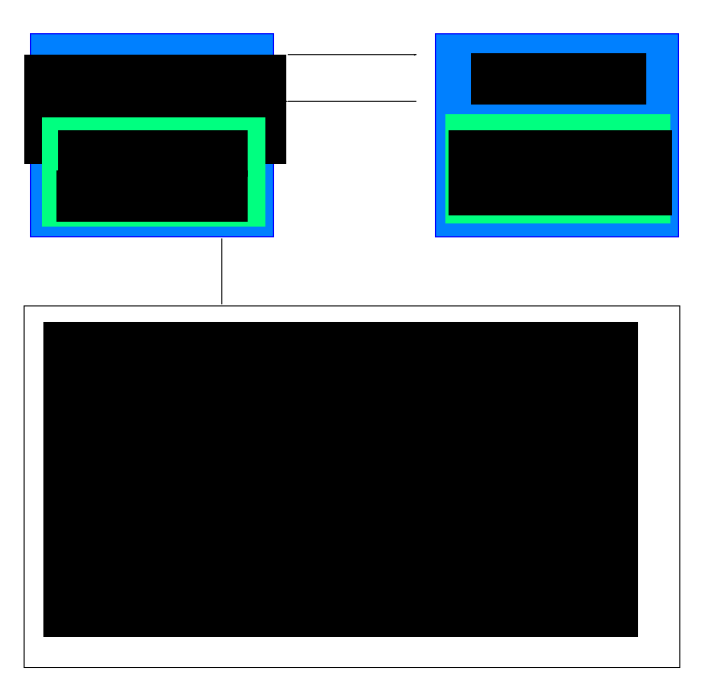
\includegraphics[width=0.4\textwidth]{arch-03.png}

  \begin{itemize}
    \item<1-> By default, devices are exposed under /dev/netchar
    \item<2-> In the future, we should be able to choose any name
  \end{itemize}
\end{frame}

\section{Implementation}

%---Code Sample Slide---%
\begin{frame}{\bf Code Sample}
  
\lstinputlisting[
  caption={Listing Code Sample},
  label=lst:codeSample.c]{codesample.c}

\end{frame}

% Matt - End

% Andy Sections

\section{Results and Evaluation}
%---Full State Slide---%

\begin{frame}[c]{Full System}
  \begin{center}
    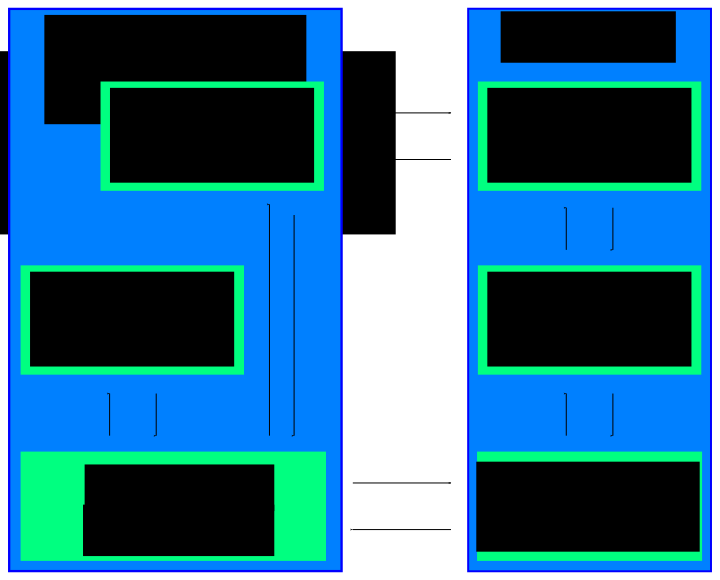
\includegraphics[height=0.75\paperheight,keepaspectratio]{system-full.png}
  \end{center}
\end{frame}

%---Current State Image Slide---%
\begin{frame}[c]{Current State}
  \begin{center}
    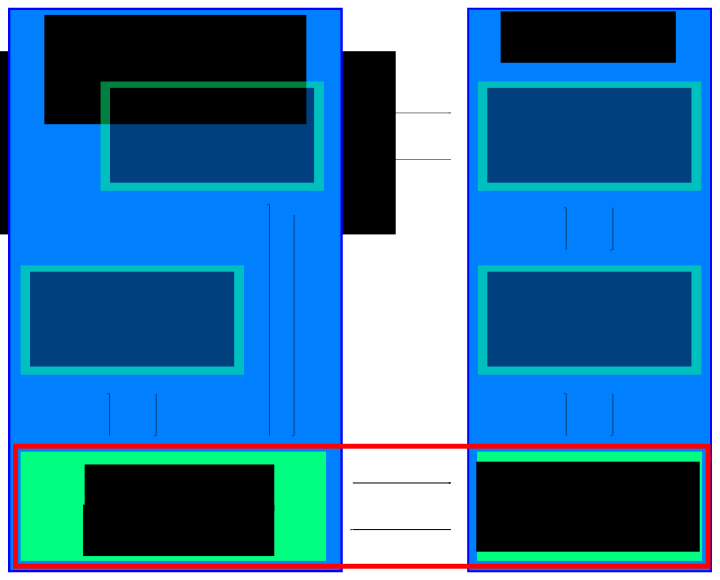
\includegraphics[height=0.75\paperheight,keepaspectratio]{system-working.png}
  \end{center}
\end{frame}

%---Current State Slide---%
\begin{frame}{\bf Current State}

\begin{itemize}
\item<1-> Supports exporting a single character device from the server
\item<2-> Supports importing a single character device on the client
\item<3-> Supports open, close, read, and write calls
\item<4-> Supports basic Linux udev operation for automatic node creation on client
\end{itemize}

\end{frame}

%---ToDo Slide---%
\begin{frame}{\bf ToDo}

\begin{itemize}
\item Multi-device, multi-server client-side import support
\item Multi-device server-side export support
\item Support for exclusive use and protection of exported devices
\item Support for ioctl calls
\item Support for providing and obtaining metadata for exported
  devices
\item Support for ``advertisement'' of available exported devices
\item Support for integrating imported devices into other kernel
  subsystems (human interface subsystem, audio subsystem, etc)
\item Addition of ``NCD-admin'' utilities for managing and administering
  NCD system
\end{itemize}

\end{frame}

%---Advantages Slide---%
\begin{frame}{\bf Advantages}

\end{frame}

%---Challenges Slide---%
\begin{frame}{\bf Challenges}

\end{frame}

\section{Future Work}

\section{Conclusion}

\section{Bibliography}
%---Bibliography---%
\begin{frame}{\bf Bibliography}

\bibliography{refs}

\end{frame}

\end{document}

% vim: set sw=2 ts=2 et : %
